% Research paper for the DWM practical - IEEE conference format (IEEEtran).
% Build: tectonic paper_dwm.tex
% Numbers: reports/final (detection) and data/warehouse.db (warehouse), see docs/WAREHOUSE.md.
\documentclass[conference]{IEEEtran}
\usepackage[T1]{fontenc}
\usepackage{cite}
\usepackage{amsmath}
\usepackage{newtxtext,newtxmath}
\usepackage{graphicx}
\usepackage{booktabs}
\usepackage{xcolor}
\usepackage{tikz}
\usetikzlibrary{arrows.meta,positioning,fit,calc}
\usepackage{url}
\usepackage[hidelinks]{hyperref}

\setlength{\textfloatsep}{8pt plus 2pt minus 2pt}
\setlength{\dbltextfloatsep}{8pt plus 2pt minus 2pt}
\setlength{\floatsep}{6pt plus 2pt minus 2pt}
\setlength{\abovecaptionskip}{3pt}

\begin{document}

\title{Sentinel: Intrusion Detection with Uncertainty-Based Analyst Review and a Data Warehouse for OLAP Analysis}

\author{
\IEEEauthorblockN{Jai Chavan, Jeet Mane, Amaan Khan}
\IEEEauthorblockA{Department of Computer Engineering\\
Vidyalankar Institute of Technology, Mumbai, India\\
jai.chavan@vit.edu.in, jeet.mane@vit.edu.in, amaan.khan@vit.edu.in}
\and
\IEEEauthorblockN{Dr. Kavita Shirsat}
\IEEEauthorblockA{Department of Computer Engineering\\
Vidyalankar Institute of Technology, Mumbai, India}
}

\maketitle

\begin{abstract}
Sentinel is a web-based prototype that combines machine-learning intrusion detection with
human judgement and with analytical storage. A convolutional-recurrent (CNN-LSTM) network assigns
each network flow to one of thirteen classes. Three checks, namely calibrated prediction entropy,
Mahalanobis distance in the network's feature space and agreement with a Random Forest, decide
whether that label is used directly or whether the flow is passed to a security analyst. Analyst
decisions are kept as searchable cases and can update the model only through admin-approved
retraining. All flows, alerts and reviews are also loaded by an extract-transform-load (ETL) job
into a dimensional data warehouse that supports roll-up, drill-down, slice, dice and pivot. On
257,222 held-out flows of the corrected CIC-IDS2017 dataset, 1.48\% of traffic was referred to
the analyst, 98.9\% of all misclassifications were among those referred flows, and the remaining
automatic decisions were 99.999\% correct. The warehouse stores 1,714,812 flows in a star schema, reloads
fully in about 25\,s, and answers frequent questions from an hourly aggregate in under a
millisecond.
\end{abstract}

\begin{IEEEkeywords}
intrusion detection, CNN-LSTM, uncertainty, human-in-the-loop, data warehouse, ETL, OLAP
\end{IEEEkeywords}

%=====================================================================
\section{Introduction}
Learning-based intrusion detectors report very high scores on public benchmarks, yet a single
score hides two practical problems. The first is that a classifier always returns some label,
including for traffic it has never encountered, so a wrong answer can look exactly as certain as
a right one. The second is that the stream of verdicts is stored for day-to-day operation, which
makes it awkward to study later, for example to see which services were attacked most or how the
workload of the analysts changed over time.

Sentinel addresses both problems in one system. For detection, the classifier is allowed to act
alone only when three independent checks agree that its answer is reliable; every other flow is
given to an analyst, whose verdict is recorded with a reason and can later be used for retraining
under administrator control. For analysis, the records are copied into a data warehouse built on
dimensional modelling \cite{inmon2005building,kimball2013toolkit}, where they can be explored with
standard OLAP operations. The warehouse only reads from the detection side, so analysis can never
alter a detection.

The main contributions are: (i) a detection pipeline that refers uncertain flows to a person and
is evaluated on untouched test data; (ii) a controlled feedback loop from analyst decisions to
model updates; and (iii) a warehouse with star, snowflake and fact-constellation schemas, full and
incremental ETL, and a browser-based OLAP cube.

%=====================================================================
\section{Related Work}
CIC-IDS2017 \cite{sharafaldin2018toward} is one of the most used flow datasets, and later work
found and repaired errors in its labels and feature extraction
\cite{engelen2021troubleshooting,liu2022error}. Common pitfalls of machine learning for security,
such as duplicated records crossing the train-test boundary and shortcut features, are discussed in
\cite{arp2022dos,sommer2010outside}. The network used here follows the hybrid CNN-LSTM design of
\cite{refpaper2025}. Its uncertainty signals draw on temperature scaling \cite{guo2017calibration},
feature-space distance for novelty detection \cite{lee2018simple} and the idea of abstaining when
unsure \cite{geifman2017selective}. On the warehousing side, the architecture and OLAP operations
follow \cite{chaudhuri1997overview} and \cite{gray1997datacube}, and the choice of a
pre-aggregated view follows \cite{harinarayan1996implementing}.

%=====================================================================
\section{System Overview}
Fig.~\ref{fig:system} shows the complete platform. Flows from the held-out test partition are
replayed through the detector to imitate live traffic. Each result is written to the operational
database as a closed flow, an alert or a review item. Analysts work through review items in a
web portal; administrators verify their decisions, run retraining and deploy or roll back model
versions. Separately, the ETL job reads the cleaned dataset and the operational database and loads
the warehouse used by the OLAP view.

\begin{figure*}[t]
\centering
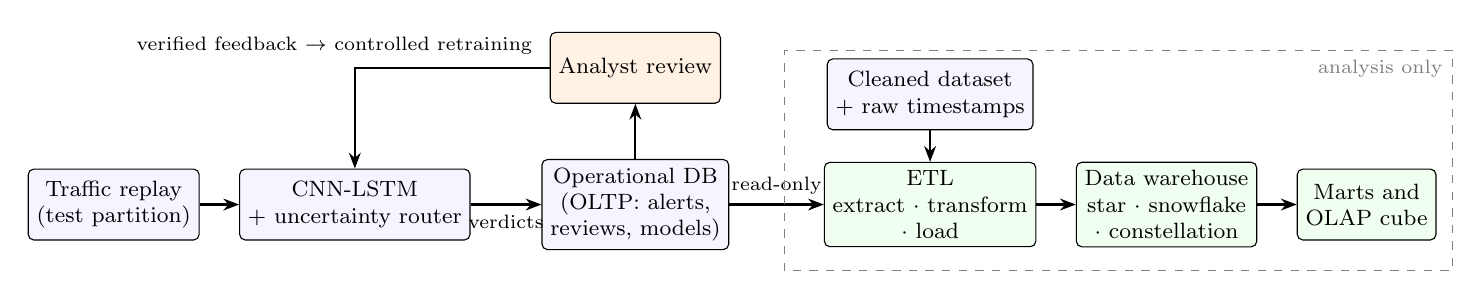
\begin{tikzpicture}[
  box/.style={draw, rounded corners=2pt, align=center, font=\footnotesize, minimum height=9mm, inner sep=3pt, fill=blue!4},
  hum/.style={box, fill=orange!10},
  dw/.style={box, fill=green!6},
  arr/.style={-{Stealth[length=2mm]}, thick},
  lab/.style={font=\scriptsize, align=center}]
\node[box] (rep) {Traffic replay\\(test partition)};
\node[box, right=5mm of rep] (det) {CNN-LSTM\\+ uncertainty router};
\node[box, right=9mm of det] (oltp) {Operational DB\\(OLTP: alerts,\\reviews, models)};
\node[hum, above=7mm of oltp] (an) {Analyst review};
\node[dw, right=12mm of oltp] (etl) {ETL\\extract $\cdot$ transform\\$\cdot$ load};
\node[box, above=4mm of etl] (src) {Cleaned dataset\\+ raw timestamps};
\node[dw, right=5mm of etl] (wh) {Data warehouse\\star $\cdot$ snowflake\\$\cdot$ constellation};
\node[dw, right=5mm of wh] (olap) {Marts and\\OLAP cube};
\draw[arr] (rep) -- (det);
\draw[arr] (det) -- node[lab, below]{verdicts} (oltp);
\draw[arr] (oltp) -- (an);
\draw[arr] (an.west) -| (det.north);
\node[lab, anchor=south east] at ($(an.west)+(-1mm,0.5mm)$) {verified feedback $\to$ controlled retraining};
\draw[arr] (oltp) -- node[lab, above]{read-only} (etl);
\draw[arr] (src) -- (etl);
\draw[arr] (etl) -- (wh);
\draw[arr] (wh) -- (olap);
\draw[dashed, gray] ($(etl.south west)+(-5mm,-3mm)$) rectangle ($(olap.north east)+(2mm,15mm)$);
\node[lab, gray, anchor=north east] at ($(olap.north east)+(2mm,15mm)$) {analysis only};
\end{tikzpicture}
\caption{Overall design. Detection and analyst review use the operational database; ETL copies
data into the warehouse for analysis only.}
\label{fig:system}
\end{figure*}

%=====================================================================
\section{Detection Method}
\subsection{Data preparation}
The corrected CIC-IDS2017 release \cite{engelen2021troubleshooting,liu2022error} has 2,099,976
flows recorded over five weekdays. The 27 raw labels were grouped into 13 classes: benign traffic
and twelve attack types (four DoS variants, DDoS, port scan, FTP and SSH password guessing, web
attacks, botnet, infiltration and Heartbleed). Fields that identify hosts or sessions (flow
identifier, IP addresses, source port, timestamp) were removed, and so was the destination port,
because it lets a model memorise where an attack was aimed instead of how it behaves. Rows that
became identical after this were merged before any split, leaving 1,714,812 flows with 64
features. The data were divided 70/15/15 with stratification. Scaling was fitted on the training
part only, and classes with fewer than 1,000 training rows were randomly oversampled to that
size so that the network did not ignore them.

\subsection{Classifier}
The network reads the 64 scaled values as a one-channel sequence. It applies a convolution with 64
filters (kernel 5) and max-pooling, a second convolution with 128 filters (kernel 3), a 128-unit LSTM
layer \cite{hochreiter1997lstm}, 30\% dropout and a final layer with one output per class. It was trained with
AdamW (learning rate $10^{-3}$, cosine decay, weight decay $10^{-4}$, batch size 1,024) for at
most 20 epochs, stopping when validation macro-F1 had not improved for four epochs. Three seeds
(42, 7 and 2025) were run. A Random Forest \cite{breiman2001random} of 100 trees and LightGBM
\cite{ke2017lightgbm} were trained on the same data as baselines.

\subsection{Deciding when to ask a person}
Half of the validation partition was used to fit the following rules; the other half was kept for
checking them. A flow is referred to the analyst if any rule fires:
\begin{itemize}
\item \textit{Entropy:} after temperature scaling ($T=1.013$), the entropy of the predicted
distribution exceeds 0.0048, the level reached by the 1\% least certain validation flows;
\item \textit{Distance:} the Mahalanobis distance of the flow's 128-value LSTM output from the
nearest class centre exceeds 1,689, the 99.5th percentile on validation data;
\item \textit{Second opinion:} the Random Forest predicts a different class, or more than 2 of its
100 trees vote against its own majority.
\end{itemize}
Flows that pass every check are closed automatically if benign or raised as confident alerts
otherwise.

\subsection{Analyst workflow and retraining}
For each referred flow the portal shows the flow's context, the top predictions, both
uncertainty values, the most unusual features and similar earlier cases. The analyst records a
decision of malicious, benign or unsure, the attack class, a reason, supporting evidence and a
confidence level. These records form a searchable knowledge repository. An administrator must
verify a record before it can be used for training. Once 20 verified records exist, a candidate
model is fine-tuned on them together with 200,000 original training rows (two epochs, learning
rate $10^{-4}$). The candidate can be approved only if, on a fixed benchmark, macro-F1 falls by
at most 0.005 and the false-positive rate rises by at most 0.0005, and if its accuracy on
held-back feedback is not lower than before. These limits were written into the configuration
before any retraining took place, and every deployed version can be rolled back.

%=====================================================================
\section{Data Warehouse and OLAP}
\subsection{Dimensional model}
The central fact table \texttt{fact\_flow} stores one row per flow (1,714,812 rows) with seven
measures: duration and the forward, backward and total counts of packets and bytes. It points to
five dimensions arranged in hierarchies: time (day, part of day, hour, minute), attack (benign or
malicious, nine categories, 13 classes), service (port range, service name, port), protocol and
data partition. Linked directly to the fact table, these form the star schema of
Fig.~\ref{fig:star}. A snowflake version moves the attack category and the calendar date into
separate tables. A fact constellation adds \texttt{fact\_alert}, one row per alert with the model's
prediction, confidence, entropy, distance and route, and \texttt{fact\_review}, a factless table
recording each analyst decision; the two share the time, attack and model dimensions. A second
factless table notes which attack classes occurred in each hour. The aggregate table
\texttt{agg\_flow\_hour} keeps hourly totals by attack class, protocol and partition in 606 rows,
and two data marts summarise threats per day and alerts per model version. The whole warehouse is
a single SQLite file of 22 tables.

\begin{figure}[t]
\centering
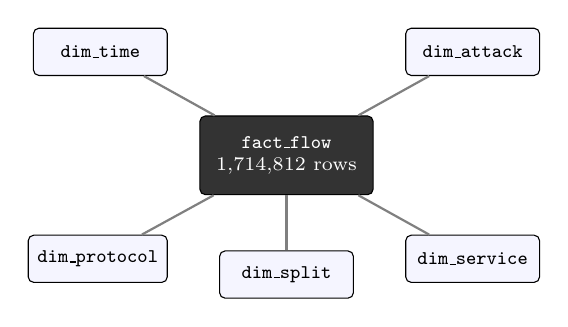
\begin{tikzpicture}[
  dim/.style={draw, rounded corners=2pt, font=\scriptsize\ttfamily, fill=blue!4, minimum width=17mm, minimum height=6mm},
  fact/.style={draw, rounded corners=2pt, font=\scriptsize, fill=black!80, text=white, align=center, minimum width=22mm, minimum height=10mm}]
\node[fact] (f) {\texttt{fact\_flow}\\1,714,812 rows};
\node[dim, above left=5mm and 4mm of f] (t) {dim\_time};
\node[dim, above right=5mm and 4mm of f] (a) {dim\_attack};
\node[dim, below left=5mm and 4mm of f] (p) {dim\_protocol};
\node[dim, below right=5mm and 4mm of f] (s) {dim\_service};
\node[dim, below=7mm of f] (sp) {dim\_split};
\foreach \n in {t,a,p,s,sp} \draw[thick, gray] (f) -- (\n);
\end{tikzpicture}
\caption{Star schema of the flow data.}
\label{fig:star}
\end{figure}

\subsection{ETL}
\emph{Extract} reads the cleaned partitions, the raw capture files for timestamps, and the
operational database through a read-only connection. \emph{Transform} matches every flow to its
raw record (all 1,714,812 matched), replaces missing or negative measures with zero, turns
timestamps into minute-level keys, maps ports to service names and classes to categories, and
assigns surrogate keys. \emph{Load} fills dimensions before facts. A full load builds a new file
and swaps it in, so readers never see a partial warehouse. An incremental load copies only alerts
with an identifier above the last stored value (the watermark). Before appending, it checks that
the alerts already loaded still match the source, so that a reset of the operational database
leads to a clean reload rather than mixed data.

\subsection{OLAP operations}
A query is described by a measure, a row dimension, an optional column dimension and filters.
Roll-up and drill-down move one level up or down a hierarchy, slice fixes one dimension to one
value, dice restricts several dimensions at once, and pivot exchanges rows and columns. The
server builds the SQL only from known table and column names and passes user values as
parameters. When a question needs nothing finer than the hour, it is answered from
\texttt{agg\_flow\_hour} instead of the full fact table. Results appear as a table, a bar chart and
a three-dimensional cube in which slices and dice are highlighted.

%=====================================================================
\section{Results}
\subsection{Classification}
Table~\ref{tab:cls} compares the models on the test partition (mean of three seeds, attack treated
as the positive class). All three are well above the values reported for the reference design.
The Random Forest is slightly more accurate than the CNN-LSTM on this split; in a run without the
LSTM layer, F1 dropped to 99.46\%, so the recurrent layer does contribute.

\begin{table}[t]
\centering
\caption{Attack-versus-benign results on the test set (\%)}
\label{tab:cls}
\setlength{\tabcolsep}{4pt}
\begin{tabular}{lrrrr}
\toprule
Model & Detection rate & Precision & F1 & Macro-F1$^\ast$ \\
\midrule
Reference \cite{refpaper2025} & 96.6 & 92.1 & 94.3 & -- \\
Random Forest & 99.92 & 99.90 & 99.91 & 99.23 \\
LightGBM & 99.91 & 99.84 & 99.88 & 99.03 \\
CNN-LSTM & 99.75 & 99.71 & 99.73 & 98.09 \\
\bottomrule
\multicolumn{5}{l}{\footnotesize $^\ast$ over the 11 classes with enough test samples}
\end{tabular}
\end{table}

\subsection{Referral to the analyst}
Table~\ref{tab:route} shows how the deployed configuration handled the 257,222 test flows. Only
3,806 flows needed a person, yet almost all of the network's mistakes were among them. To see what
happens with attacks that are absent from training, each attack family was removed from the
training data in turn. On its own, the network silently closed 97.0\% of unseen web attacks,
39.7\% of unseen port scans and 12.4\% of unseen botnet flows; with the three checks these shares
fell to 5.0\%, 4.3\% and 10.2\%. SSH password guessing was not caught, because each login
attempt on its own looks like normal traffic.

\begin{table}[t]
\centering
\caption{Handling of 257,222 test flows}
\label{tab:route}
\begin{tabular}{lrr}
\toprule
Outcome & Flows & Share \\
\midrule
Closed automatically & 212,015 & 82.4\% \\
Confident alert & 41,401 & 16.1\% \\
Referred to analyst & 3,806 & 1.48\% \\
\midrule
Network errors inside the referred set & \multicolumn{2}{r}{98.9\%} \\
Accuracy of automatic decisions & \multicolumn{2}{r}{99.999\%} \\
Attacks closed as benign / benign alerted & \multicolumn{2}{r}{2 / 0} \\
\bottomrule
\end{tabular}
\end{table}

\subsection{Warehouse performance and findings}
A full ETL load took about 25\,s and an incremental load with no new alerts about 0.3\,s. The
question ``flows per day and attack class'' took about 2.3\,s on \texttt{fact\_flow} and about
0.3\,ms on the hourly aggregate. On the same category-per-day question the star schema needed
2,046\,ms and the snowflake 2,312\,ms, because of its extra joins.

The OLAP view also describes the dataset itself. Rolling up to categories shows that Monday has
no attacks, Wednesday carries 177,506 denial-of-service flows and Friday 95,144 DDoS flows.
Drilling Wednesday down to hours places 158,662 of those DoS flows in a single hour. A slice on
the service dimension shows that 94.4\% of all attack flows used HTTP, while benign traffic is
mostly DNS and HTTPS. After a replay session, an incremental load brings the portal's alerts
and reviews into the alert cube, where the routing behaviour can be inspected in the same way.

%=====================================================================
\section{Conclusion}
Sentinel shows that a detector does not have to choose between full automation and manual
checking. By referring only the 1.48\% of flows it is unsure about, it keeps automatic decisions
almost error-free and turns most unseen attacks into analyst cases. The data warehouse gives the
same data a second use: flows, alerts and reviews can be summarised and explored with OLAP
operations without touching the detector. Future work includes features computed over many flows
of a host to catch slow attacks such as SSH password guessing, retraining the Random Forest along
with the network, and loading the CSE-CIC-IDS2018 dataset into the same schema.

\section*{Acknowledgment}
The authors thank Dr. Kavita Shirsat for her guidance throughout this project.

%=====================================================================
\begin{thebibliography}{99}

\bibitem{inmon2005building}
W.~H. Inmon, \textit{Building the Data Warehouse}, 4th~ed. Indianapolis, IN, USA: Wiley, 2005.

\bibitem{kimball2013toolkit}
R.~Kimball and M.~Ross, \textit{The Data Warehouse Toolkit: The Definitive Guide to Dimensional Modeling}, 3rd~ed. Indianapolis, IN, USA: Wiley, 2013.

\bibitem{sharafaldin2018toward}
I.~Sharafaldin, A.~H. Lashkari, and A.~A. Ghorbani, ``Toward generating a new intrusion detection dataset and intrusion traffic characterization,'' in \textit{Proc. 4th Int. Conf. Information Systems Security and Privacy (ICISSP)}, 2018, pp. 108--116.

\bibitem{engelen2021troubleshooting}
G.~Engelen, V.~Rimmer, and W.~Joosen, ``Troubleshooting an intrusion detection dataset: the CICIDS2017 case study,'' in \textit{Proc. IEEE Security and Privacy Workshops (SPW)}, 2021, pp. 7--12.

\bibitem{liu2022error}
L.~Liu, G.~Engelen, T.~Lynar, D.~Essam, and W.~Joosen, ``Error prevalence in NIDS datasets: A case study on CIC-IDS-2017 and CSE-CIC-IDS-2018,'' in \textit{Proc. IEEE Conf. Communications and Network Security (CNS)}, 2022, pp. 254--262.

\bibitem{arp2022dos}
D.~Arp \textit{et al.}, ``Dos and don'ts of machine learning in computer security,'' in \textit{Proc. 31st USENIX Security Symposium}, 2022, pp. 3971--3988.

\bibitem{sommer2010outside}
R.~Sommer and V.~Paxson, ``Outside the closed world: On using machine learning for network intrusion detection,'' in \textit{Proc. IEEE Symposium on Security and Privacy}, 2010, pp. 305--316.

\bibitem{refpaper2025}
C.~M. de~Nascimento and J.~Hou, ``Uncertainty-aware adaptive intrusion detection using hybrid CNN-LSTM with cWGAN-GP augmentation and human-in-the-loop feedback,'' \textit{Safety}, vol.~11, no.~4, Art.~no.~120, Dec. 2025.

\bibitem{guo2017calibration}
C.~Guo, G.~Pleiss, Y.~Sun, and K.~Q. Weinberger, ``On calibration of modern neural networks,'' in \textit{Proc. 34th Int. Conf. Machine Learning (ICML)}, 2017, pp. 1321--1330.

\bibitem{lee2018simple}
K.~Lee, K.~Lee, H.~Lee, and J.~Shin, ``A simple unified framework for detecting out-of-distribution samples and adversarial attacks,'' in \textit{Advances in Neural Information Processing Systems (NeurIPS)}, 2018, pp. 7167--7177.

\bibitem{geifman2017selective}
Y.~Geifman and R.~El-Yaniv, ``Selective classification for deep neural networks,'' in \textit{Advances in Neural Information Processing Systems (NeurIPS)}, 2017, pp. 4878--4887.

\bibitem{chaudhuri1997overview}
S.~Chaudhuri and U.~Dayal, ``An overview of data warehousing and OLAP technology,'' \textit{ACM SIGMOD Record}, vol.~26, no.~1, pp. 65--74, 1997.

\bibitem{gray1997datacube}
J.~Gray \textit{et al.}, ``Data cube: A relational aggregation operator generalizing group-by, cross-tab, and sub-totals,'' \textit{Data Mining and Knowledge Discovery}, vol.~1, no.~1, pp. 29--53, 1997.

\bibitem{harinarayan1996implementing}
V.~Harinarayan, A.~Rajaraman, and J.~D. Ullman, ``Implementing data cubes efficiently,'' in \textit{Proc. ACM SIGMOD Int. Conf. Management of Data}, 1996, pp. 205--216.

\bibitem{hochreiter1997lstm}
S.~Hochreiter and J.~Schmidhuber, ``Long short-term memory,'' \textit{Neural Computation}, vol.~9, no.~8, pp. 1735--1780, 1997.

\bibitem{breiman2001random}
L.~Breiman, ``Random forests,'' \textit{Machine Learning}, vol.~45, no.~1, pp. 5--32, 2001.

\bibitem{ke2017lightgbm}
G.~Ke \textit{et al.}, ``LightGBM: A highly efficient gradient boosting decision tree,'' in \textit{Advances in Neural Information Processing Systems (NeurIPS)}, 2017, pp. 3146--3154.

\end{thebibliography}

\end{document}
